%% KSPFail — IEEE two-column conference paper
%% Ported from docs/paper_full_draft.md (content-locked). Build: pdflatex kspfail.tex (x2).
%% Figures referenced relative to this file: ../results/figures/ and ../results/ml-first-pass/
\documentclass[conference]{IEEEtran}
\IEEEoverridecommandlockouts
\usepackage{cite}
\usepackage{amsmath,amssymb,amsfonts}
\usepackage{graphicx}
\usepackage{textcomp}
\usepackage{xcolor}
\usepackage{booktabs}
\usepackage{array}
\usepackage{url}

% Fault-class name shorthands (keeps underscores correctly escaped everywhere)
\newcommand{\bk}{broker\_kill}
\newcommand{\eo}{executor\_oom}
\newcommand{\dpr}{disk\_pressure}
\newcommand{\nd}{network\_degradation}
\newcommand{\bc}{backpressure\_cascade}
\newcommand{\yes}{\checkmark}
\newcommand{\no}{--}
\newcommand{\pmark}{$\sim$}

\begin{document}

\title{A Fault-Injection Benchmark for Lead-Time Failure Prediction on Kafka--Spark Structured Streaming Pipelines}

\author{
\IEEEauthorblockN{1\textsuperscript{st} Renold Stephen R}
\IEEEauthorblockA{\textit{Dept. of Computer Science and Engineering} \\
\textit{Christ University}\\
Bangalore, India \\
renold.stephen@mtech.christuniversity.in}
\and
\IEEEauthorblockN{2\textsuperscript{nd} H. Karthikeyan}
\IEEEauthorblockA{\textit{Dept. of Computer Science and Engineering} \\
\textit{Christ University}\\
Bangalore, India \\
karthikeyan.h@christuniversity.in}
\and
\IEEEauthorblockN{3\textsuperscript{rd} Diana Jeba Jingle I}
\IEEEauthorblockA{\textit{Dept. of Computer Science and Engineering} \\
\textit{Christ University}\\
Bangalore, India \\
diana.jebajingle@christuniversity.in}
}

\maketitle

\begin{abstract}
Kafka and Spark Structured Streaming pipelines are core data infrastructure, and their failures---broker crashes, executor out-of-memory kills, disk exhaustion, network degradation---are caught in current practice by static-threshold alerting that fires only after degradation is visible. Whether supervised machine learning on pre-failure telemetry can warn earlier, and by how much, has not been benchmarked for this pipeline layer specifically. We build a reproducible fault-injection benchmark on a live Kafka + Spark Structured Streaming pipeline instrumented with Prometheus, physically inject five fault classes with onset timestamps recorded by the injection tooling itself, and construct a labeled dataset of 47 fault episodes (102 telemetry windows). We compare three tree-based classifiers (Random Forest, XGBoost, LightGBM) under leave-one-group-out cross-validation against a static-threshold baseline that reproduces real alerting practice, using rank-based permutation testing and a lead-time metric. Only one of five fault classes produces a classification signal that clears chance-level significance (F1 = 0.941, $p < 0.01$); per-instance ablation and SHAP show even this is an absolute-value discriminator, not detection of a physical precursor. No class yields a machine-learning lead-time advantage over the threshold baseline---a null result that holds across all three classifiers and does not move when one class is enlarged from 8 to 15 episodes. The contribution is the open benchmark, the labeled dataset, and a mechanism-verification methodology that catches such over-claims before they are reported.
\end{abstract}

\begin{IEEEkeywords}
AIOps, fault injection, failure prediction, Apache Kafka, Spark Structured Streaming, lead time, benchmark, static-threshold alerting
\end{IEEEkeywords}

\section{Introduction}
Streaming data infrastructure---Apache Kafka \cite{kreps2011} for ingestion and Spark Structured Streaming \cite{armbrust2018} for processing---underpins modern data platforms, and its reliability is operationally critical: a stalled consumer group or a crashed broker degrades downstream data freshness long before an operator notices. The dominant operational response is threshold-based alerting: fire when consumer lag exceeds a bound, or when under-replicated partitions rise above zero. This is reactive by construction---the threshold is crossed only once degradation is already under way.

Proactive failure prediction has been the alternative premise for over a decade \cite{salfner2010}. The AI-for-IT-operations (AIOps) literature has established, across general distributed-systems settings, that machine-learning (ML) models trained on system telemetry can anticipate failures earlier than static rules \cite{notaro2021,zhang2024}. This has been shown concretely in adjacent domains: DRAM failure prediction at data-center scale \cite{wu2021}, node-failure prediction in cloud service systems \cite{lin2018}, and batch-cluster job-failure prediction \cite{harrison2018}. One recent system predicts both failure and its lead time, though on high-performance-computing (HPC) logs rather than streaming telemetry \cite{alharthi2023}. What has not been benchmarked with the same rigor is the specific combination of controlled fault injection, multi-model comparison, and lead-time evaluation applied to a Kafka + Spark Structured Streaming pipeline as the object of prediction---as distinct from anomaly detection on the data flowing \emph{through} the pipeline, and from Spark job runtime prediction, both of which are separately studied.

This paper reports that benchmark, and its result is a cautionary one. Across five physically injected fault classes, only one produces a classification signal that survives a permutation test against chance, and closer inspection shows that signal is not the early-warning capability it superficially resembles. No fault class yields a machine-learning lead-time advantage over a static-threshold baseline that reproduces current practice. We report this negative result with the same rigor as a positive one, because the value here is the measurement apparatus and what it honestly finds, not a model that wins.

The contributions are:
\begin{itemize}
\item A reproducible, open fault-injection benchmark on a live Kafka + Spark Structured Streaming pipeline, with infrastructure-as-code, five injection scripts, and a static-threshold baseline reproducing current alerting practice.
\item A labeled dataset of 47 real fault episodes across five classes, each carrying an onset timestamp recorded by the injection tooling at the moment it caused the fault---not inferred or human-annotated afterward---with paired Prometheus telemetry that makes lead-time computation possible.
\item A lead-time evaluation and multi-model comparison (Random Forest, XGBoost, LightGBM) against the threshold baseline, showing no ML lead-time advantage on this pipeline for any class.
\item A mechanism-verification methodology---per-instance ablation and SHAP cross-checking applied to every positive-looking result before it is trusted---which caught this study's one significant classification result as an absolute-value discriminator rather than genuine precursor detection.
\end{itemize}

No contribution here is a novel model or algorithm; every classifier is a stock implementation with standard hyperparameters. The contribution is the benchmark, the dataset, and the measurement discipline. Section~\ref{sec:related} positions the work; Section~\ref{sec:method} describes the infrastructure, fault taxonomy, dataset, baseline, and evaluation; Section~\ref{sec:results} reports results; Section~\ref{sec:discussion} discusses them; and Section~\ref{sec:conclusion} concludes.

\section{Related Work}\label{sec:related}
\textbf{Failure prediction in distributed systems.} Online failure prediction---using runtime telemetry to flag impending failure---has a well-developed taxonomy \cite{salfner2010}, and AIOps surveys establish ML-over-thresholds as a mature premise across IT operations \cite{notaro2021,zhang2024}. Concrete demonstrations exist in adjacent domains: an empirical multi-classifier benchmark for DRAM failures \cite{wu2021}, a Random-Forest job-failure predictor on HPC batch clusters reaching 95.4\% accuracy \cite{harrison2018}, and MING, which predicts node failures in Microsoft cloud systems at 63.5\% recall and 92.4\% precision \cite{lin2018}. These establish that the method works---but in hardware, batch-scheduling, and node-level settings, none on a streaming-pipeline layer, and none reporting a lead-time metric except in HPC logs.

\textbf{Lead-time prediction.} The closest thematic neighbor is Time Machine \cite{alharthi2023}, which predicts failure, its location, and its lead time using a transformer-decoder over HPC event logs. It shares our target---lead time as an explicit prediction quantity---but differs on every axis that matters here: it learns from naturally occurring failures rather than controlled injection, operates on log events rather than Prometheus telemetry, compares against deep-learning baselines rather than a static-threshold detector, and contributes a model rather than a benchmark.

\textbf{Fault injection and chaos engineering.} Deliberately inducing faults to study system behavior is an established experimental discipline \cite{basiri2016}, surveyed comprehensively for software fault injection \cite{natella2016}. Recent work injects node-, pod-, and network-level faults into live Kubernetes clusters and measures application-level resilience \cite{chen2025}. Our injection methodology sits in this lineage, but where \cite{chen2025} measures post-fault resilience, we convert injection output into a labeled dataset for predictive modeling.

\textbf{Streaming-pipeline reliability benchmarks.} The nearest systems benchmark injects chaos-style faults across Flink, Kafka Streams, and Spark Structured Streaming and compares fault-recovery performance \cite{vogel2024}. It shares our substrate---Kafka and Spark on Kubernetes with injected faults---but answers a different question: post-hoc recovery speed across competing engines, not predictive lead time on a fixed pipeline. It reports no labeled pre-failure dataset and no static-threshold-versus-ML comparison. Separately, gray-box modeling predicts Spark job \emph{runtime} \cite{alsayeh2020}; this sharpens rather than competes with our framing---predicting execution time is a distinct, solved problem from predicting failure. The open-benchmark-plus-reproducible-baselines pattern we follow is exemplified in microservice root-cause analysis by RCAEval \cite{pham2025}, though that addresses post-hoc diagnosis rather than prediction.

Table~\ref{tab:related} makes the gap explicit: no located work combines controlled fault injection, multi-model ML, lead-time evaluation, and a static-threshold baseline on a fixed Kafka + Spark Structured Streaming pipeline. Each prior work satisfies some criteria; none satisfies all.

\begin{table*}[!t]
\caption{Positioning against prior work. \yes: fully addressed; \pmark: partial; \no: not addressed. Only this work satisfies all six criteria.}
\label{tab:related}
\centering
\footnotesize
\begin{tabular}{@{}lcccccc@{}}
\toprule
\textbf{Work} & \textbf{Fault injection} & \textbf{ML failure pred.} & \textbf{Lead-time eval.} & \textbf{Threshold baseline} & \textbf{Kafka+Spark SS} & \textbf{Open dataset} \\
\midrule
Wu et al.\ \cite{wu2021}          & \no  & \yes & \no  & \no & \no  & \pmark \\
Harrison et al.\ \cite{harrison2018} & \no  & \yes & \no  & \no & \no  & \no \\
Lin et al.\ \cite{lin2018}        & \no  & \yes & \no  & \no & \no  & \no \\
Alharthi et al.\ \cite{alharthi2023} & \no  & \yes & \yes & \no & \no  & \pmark \\
Basiri et al.\ \cite{basiri2016}  & \yes & \no  & \no  & \no & \no  & \no \\
Chen et al.\ \cite{chen2025}      & \yes & \no  & \no  & \no & \no  & \pmark \\
Vogel et al.\ \cite{vogel2024}    & \yes & \no  & \no  & \no & \yes & \yes \\
Al-Sayeh et al.\ \cite{alsayeh2020} & \no & \pmark & \no & \no & \pmark & \no \\
\textbf{This work}                & \yes & \yes & \yes & \yes & \yes & \yes \\
\bottomrule
\end{tabular}
\end{table*}

\section{Methodology}\label{sec:method}
\subsection{System Under Test and Infrastructure}
The pipeline runs on a single-node Kind Kubernetes cluster: a single Strimzi-managed Kafka broker (Kafka 4.3.0) with a JMX exporter, a Spark 4.1.2 Structured Streaming job (driver plus executors) consuming from Kafka, and a continuous producer generating load. Prometheus scrapes three metric sources on a 60-second interval---the broker's JMX exporter, cAdvisor container metrics, and node-exporter host metrics. Fig.~\ref{fig:arch} shows the topology and the five fault-injection points. The entire stack is declarative infrastructure-as-code, reproducible from the repository without a running cluster; the injection scripts operate against this live deployment. A single-node cluster is a deliberate scope choice---it makes the benchmark reproducible on a laptop-class machine, at the cost of the external-validity limitation discussed in Section~\ref{sec:discussion}.

\begin{figure*}[!t]
\centering
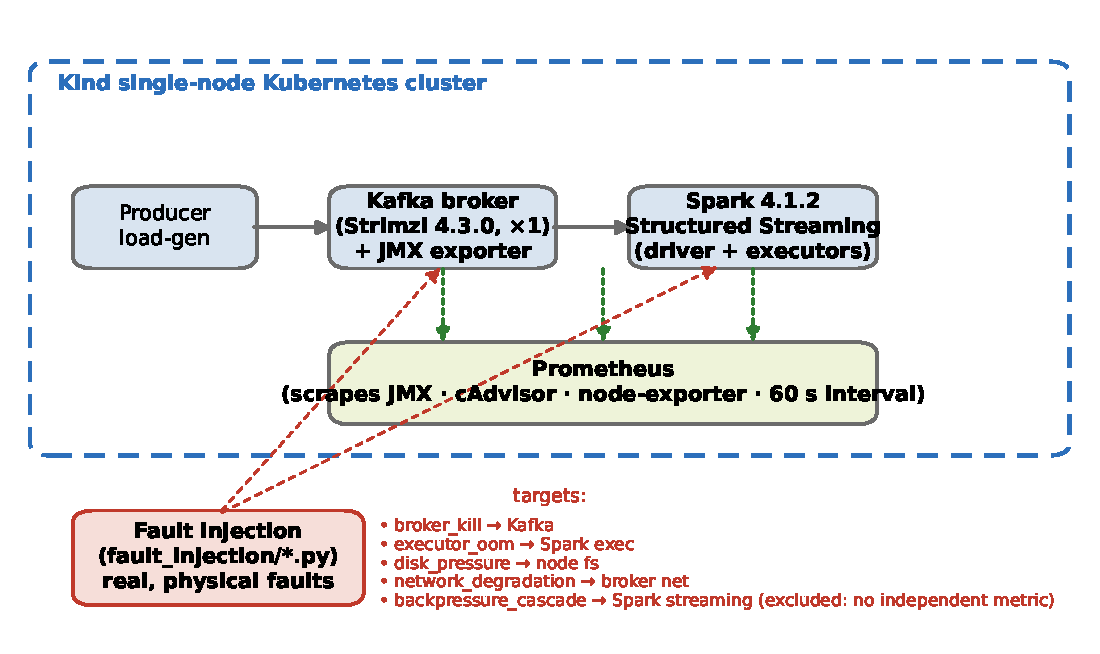
\includegraphics[width=0.92\textwidth]{figures/fig1-architecture.pdf}
\caption{System under test---single-node Kind cluster with Strimzi Kafka, Spark Structured Streaming, and Prometheus (60\,s scrape)---and the five fault-injection points.}
\label{fig:arch}
\end{figure*}

\subsection{Fault Taxonomy and Injection}
Five fault classes are injected, chosen to span Kafka-side, Spark-side, and node-level failure modes reproducible on a single node (Table~\ref{tab:taxonomy}). Each is a real, physical fault: \bk{} deletes the broker pod; \eo{} drives a Spark executor's memory up a gradual ramp until the Kubernetes OOM killer fires; \dpr{} fills the node filesystem; \nd{} applies \texttt{tc netem} delay, jitter, and loss to the broker; \bc{} bursts producer load to induce consumer lag. Each injection script records its own ground-truth timestamps---injection onset and a class-specific confirmation event---at the moment it acts, so labels derive from the tooling's own record rather than post-hoc inference.

The static-threshold rule for each class is grounded in this pipeline's own observed telemetry, not borrowed from an industry rule of thumb: thresholds sit with real margin between the measured baseline and the measured fault-window value (Table~\ref{tab:taxonomy}). \bc{} is injected and its ground truth recorded, but excluded from modeling: no independently scraped Prometheus metric reflects Spark processing lag on this deployment---the only available lag field is the driver-log-parsed one the ground truth itself uses, so any detector built from it would be circular.

\begin{table*}[!t]
\caption{Fault taxonomy: the five injected classes, their injection mechanism, target, monitored Prometheus signal, and static-threshold rule.}
\label{tab:taxonomy}
\centering
\footnotesize
\begin{tabular}{@{}lllll@{}}
\toprule
\textbf{Fault class} & \textbf{Injection mechanism} & \textbf{Target} & \textbf{Prometheus signal} & \textbf{Static threshold} \\
\midrule
\bk{}  & Delete the broker pod (outage)          & Kafka broker      & \texttt{up} target-down                       & binary target-down \\
\eo{}  & Gradual memory ramp to OOM kill         & Spark executor    & \texttt{container\_memory\_working\_set\_bytes} & $>900$\,MB ($\approx$75\% of limit) \\
\dpr{} & One-shot 3\,GB fill of \texttt{/var}    & Node filesystem   & \texttt{node\_filesystem\_avail\_bytes}       & $\Delta$-drop $>1.5$\,GB \\
\nd{}  & \texttt{tc netem} delay+jitter+loss, 90\,s & Broker network  & \texttt{scrape\_duration\_seconds}            & $>1.5$\,s \\
\bc{}  & Burst load $\rightarrow$ consumer lag   & Spark streaming   & none independently scraped                    & N/A (excluded) \\
\bottomrule
\end{tabular}
\end{table*}

\subsection{Dataset Construction and Labeling}
The campaign yields 47 active fault episodes and 20 discarded ones, every exclusion carrying a per-episode recorded reason (Table~\ref{tab:dataset}). Feature extraction produces 102 labeled telemetry windows across the four modeled classes. For each window, six raw statistics (mean, standard deviation, min, max, last value, sample count) are computed over the metric most relevant to that fault class; delta features expressing each statistic relative to the episode's own pre-injection baseline are derived on top. Pre-failure windows are drawn from the horizon immediately before each episode's recorded onset; normal windows come either from a genuinely quiet reference period or, for the pod-scoped \eo{} class, from each episode's pre-injection settling period. The window/horizon configuration (15-second windows ending 10--15 seconds before onset) was selected after a four-point sensitivity sweep showed wider configurations were not contamination-safe at the tightest real inter-episode gaps.

\begin{table*}[!t]
\caption{Dataset summary: active/discarded episode counts per class with discard reasons, ground-truth confirmation field, and modeling window counts.}
\label{tab:dataset}
\centering
\footnotesize
\begin{tabular}{@{}lccllc@{}}
\toprule
\textbf{Fault class} & \textbf{Active} & \textbf{Discarded} & \textbf{Discard reason (summary)} & \textbf{Ground-truth field} & \textbf{Windows} \\
\midrule
\bk{}  & 8  & 0  & ---                                       & \texttt{target\_recovered\_utc}        & 26 \\
\eo{}  & 15 & 10 & superseded instant-onset design; config-fix window & \texttt{oomkilled\_confirmed\_utc} & 24 \\
\dpr{} & 8  & 1  & drop not confirmed within polling window   & \texttt{drop\_confirmed\_utc}          & 26 \\
\nd{}  & 8  & 8  & timeout-censored reps (since-fixed harness) & \texttt{degraded\_health\_detected\_utc} & 26 \\
\bc{}  & 8  & 1  & provenance gap (config-bug risk window)    & \texttt{caught\_up\_utc}               & 0 \\
\midrule
\textbf{Total} & \textbf{47} & \textbf{20} & every exclusion reason recorded & --- & \textbf{102} \\
\bottomrule
\end{tabular}
\end{table*}

\subsection{Static-Threshold Baseline}
The baseline reproduces current alerting practice: a detector fires when the class's metric crosses its threshold (Table~\ref{tab:taxonomy}). It is evaluated on the same episodes as the models---detection recall and lead time on the 8 active reps per class, and false-positive rate on the deliberate inter-episode steady-state gaps. Thresholds are calibrated against these same episodes' observed values; this is standard for a baseline meant to mirror how an operations team tunes its own alerts, but it means the baseline's recall reflects fit to its calibration data, not out-of-sample generalization---stated plainly as a limitation rather than hidden.

\subsection{Models, Evaluation, and Significance Testing}
Three stock tree-based classifiers are compared: Random Forest \cite{breiman2001}, XGBoost \cite{chen2016}, and LightGBM \cite{ke2017}. The reported configuration is \texttt{RandomForestClassifier} with 200 estimators, maximum depth 5, and balanced class weighting; class weighting addresses the pre-failure/normal imbalance. Because episodes are the unit of independence, all evaluation uses leave-one-group-out (LOO) cross-validation grouped by episode, so no window from a test episode appears in training. Two guards protect against over-reading. First, every result is tested for significance by a rank-based permutation test: the identical pipeline is re-run on 100 label-shuffled datasets, and the $p$-value is the fraction scoring an F1 at or above the real result. Second, any positive-looking result is subjected to mechanism verification---per-instance ablation to locate the classifier's actual decision boundary, and SHapley Additive exPlanations (SHAP) \cite{lundberg2017} attribution over the real cross-validation folds---before it is reported as evidence of early detection. Lead time, where computable, is measured by a contamination-safe backward scan from injection onset, bounded by the real measured gap to the nearest preceding episode of any class.

\section{Results}\label{sec:results}
Table~\ref{tab:results} summarizes classification and lead-time outcomes across the five fault classes. Two results need methodological unpacking before they can be read at face value, and both are addressed below.

\begin{table*}[!t]
\caption{Classification and lead-time outcomes. F1 and $p$ are from leave-one-group-out cross-validation with rank-based permutation testing (100 shuffles), on each class's corrected feature set. Baseline lead time is the static-threshold detector's own reported lead.}
\label{tab:results}
\centering
\footnotesize
\begin{tabular}{@{}lcclll@{}}
\toprule
\textbf{Fault class} & \textbf{F1} & \textbf{Perm.\ $p$} & \textbf{Baseline lead time} & \textbf{ML lead time} & \textbf{Verdict} \\
\midrule
\dpr{} & 0.941 & $<0.01$ & 0.0\,s (8/8)                       & see \S\ref{sec:results}-B & Significant, but mischaracterized \\
\bk{}  & 0.762 & 0.25    & N/A (recall 12.5\%)               & not computed              & No validated signal \\
\nd{}  & 0.118 & 1.00    & 0\,s$\times$3, 65\,s$\times$1 (4/8) & not computed             & No validated signal \\
\eo{}  & 0.909 & 0.500   & 64.9\,s (48--83\,s)               & not computed              & No validated signal ($N{=}15$) \\
\bc{}  & \multicolumn{2}{c}{not modeled} & excluded                & not computed              & No comparison possible \\
\bottomrule
\end{tabular}
\end{table*}

\subsection{Classification Performance Across Fault Classes}
Of the five classes, only \dpr{} clears permutation-test significance. \bk{}'s full feature set produced an uncorrected F1 of 0.667, but feature-importance inspection found the sample-count feature carrying 100\% of the model's importance---the availability metric this class scrapes is flat regardless of window position, so only the incidental sample-count parity between pre-failure and normal windows was driving classification. Removing that feature drops the score to F1 = 0.762 (precision 0.615, recall 1.000), which the permutation test places at chance ($p = 0.25$). This null is not a weak-model artifact: at the pipeline's 60-second scrape interval, the class's own ground truth captured an in-fault telemetry sample in only 1 of 8 episodes, so most labeled pre-failure windows have no observable signal to learn from. \nd{} is negative under the full feature set (F1 = 0.414); a shape-only (standard-deviation) ablation returns F1 = 0.118, below all 100 shuffled reruns ($p = 1.00$), the cleanest negative in the study. Model choice does not change any verdict: Random Forest, XGBoost, and LightGBM agree per class under nested-tuned LOO-CV.

\subsection{\texttt{disk\_pressure}: A Significant but Mischaracterized Signal}
\dpr{} is the only class clearing significance: F1 = 0.941 (precision 0.889, recall 1.000) using delta features, with 0 of 100 shuffled reruns matching the real F1 ($p < 0.01$). A result this clean warranted checking \emph{what} the classifier had learned. Per-instance ablation swept each held-out fold's delta feature to the value at which its prediction flips; all seven ablated folds located this boundary at the same value, $-350{,}000$ bytes, with zero variation---the signature of a static absolute-value check, not a graded response to an escalating quantity. A SHAP analysis of the same LOO models corroborates this independently: across all 16 true-positive windows, the four magnitude features carry 97.4\% of mean absolute attribution (Fig.~\ref{fig:shap}). The raw delta values at the classifier's trained decision horizons are uniformly non-negative---available disk space had not begun declining at any window the classifier saw---so there was no downward trend for any feature to detect. The classifier distinguishes ``\dpr{} recording session'' from ``quiet reference period'' on an absolute-value basis; that distinction is real and statistically significant, but it is not detection of the injected fault's physical precursor, whose true magnitude (a 3.22\,GB drop) is three to four orders of magnitude larger than the $\approx$350\,KB margin the classifier relies on.

\begin{figure}[!t]
\centering
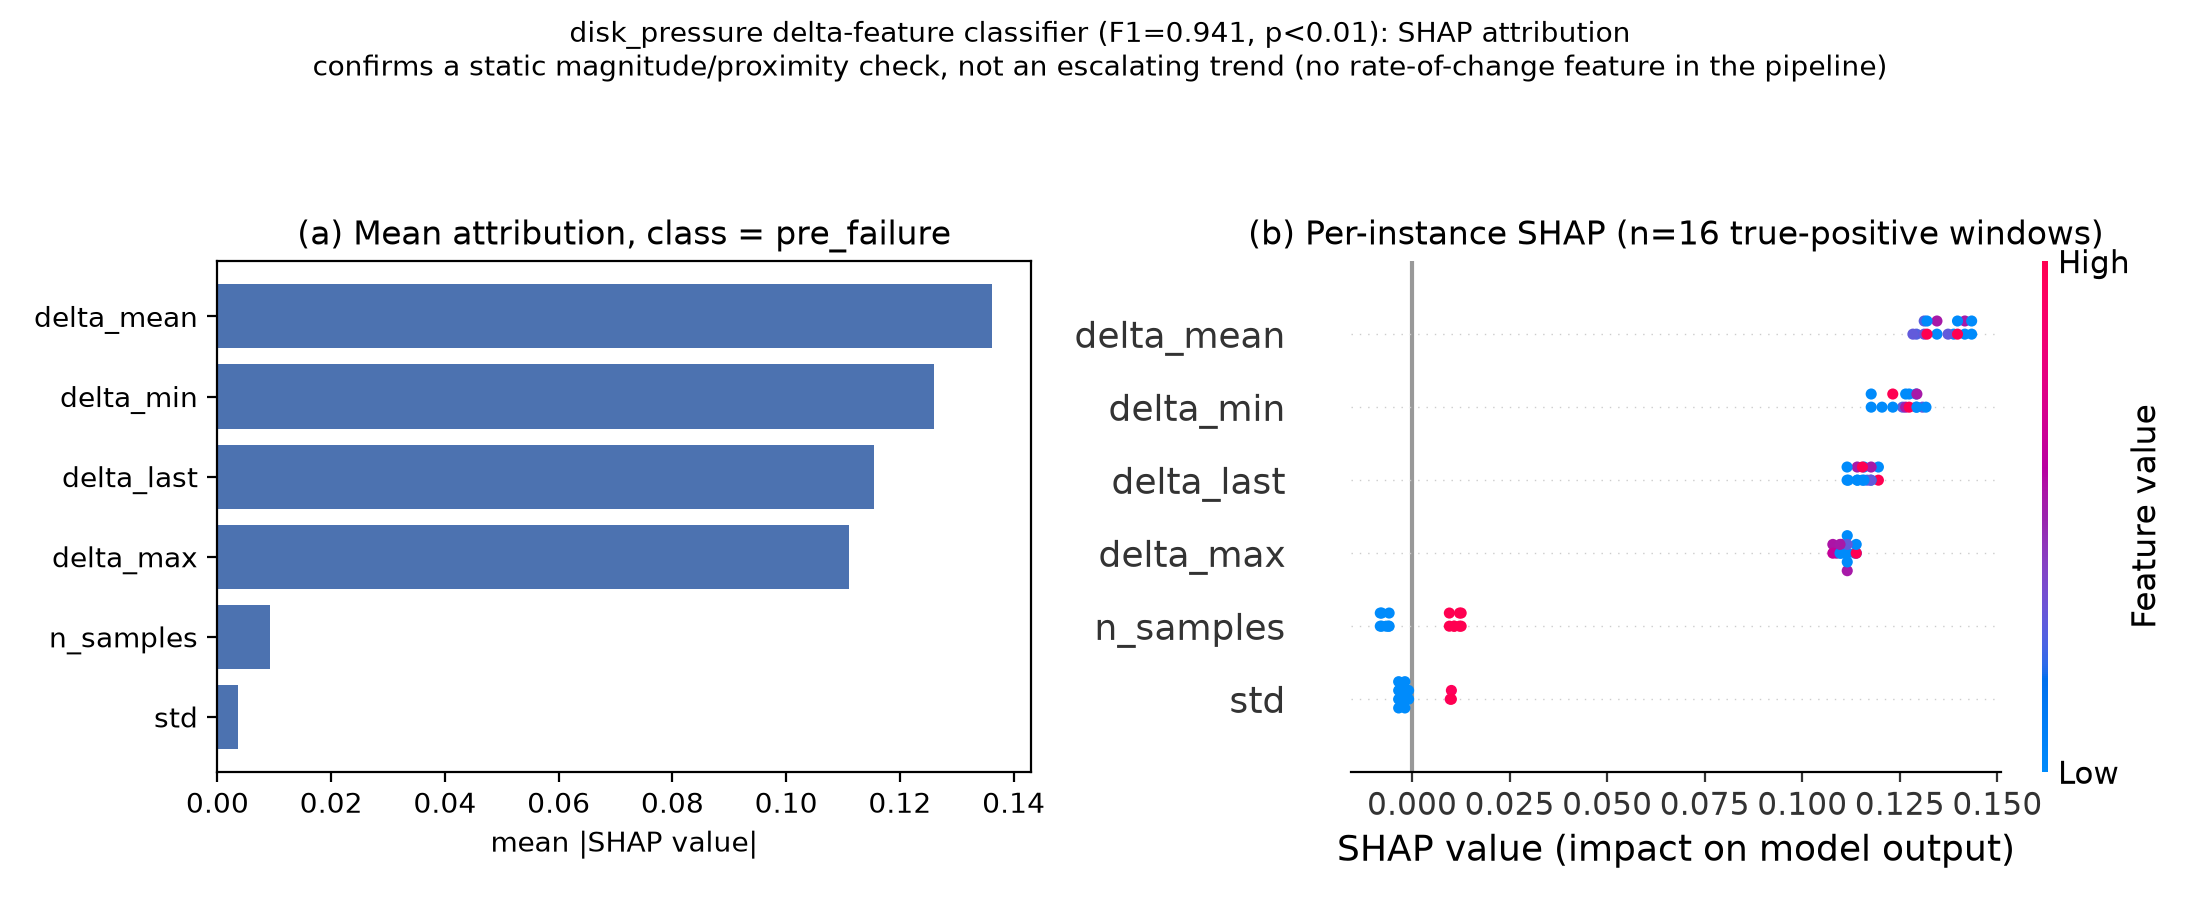
\includegraphics[width=\columnwidth]{figures/fig2-shap.png}
\caption{SHAP attribution for the \dpr{} delta-feature classifier (F1 = 0.941, $p < 0.01$) across all 16 true-positive windows: the four magnitude features carry 97.4\% of attribution, the fingerprint of an absolute-value discriminator rather than trend detection.}
\label{fig:shap}
\end{figure}

\subsection{Lead-Time Evaluation}
The central question is whether models predict failure with a meaningful lead time relative to the threshold baseline. Only \eo{}'s deliberately engineered gradual ramp yields a consistent baseline lead: the threshold crosses a mean 64.9 seconds before the OOM kill (range 48--83\,s across 8 reps), because the ramp produces real intermediate samples (Fig.~\ref{fig:lead}). \dpr{} and \nd{} collapse to $\approx$0\,s---their telemetry jumps from baseline to full fault magnitude in a single 60-second scrape step, leaving no intermediate sample; \nd{} additionally reaches its severity bar in only 4 of 8 reps. \bk{}'s baseline is not a lead time at all: for a binary up/down signal, threshold crossing coincides with the outage, and detection recall is 12.5\% at this scrape interval.

On the ML side, no class supports a positive lead-time claim. Three classes produced no significant classification signal, so no lead time was computed---reporting one for a chance-level classifier would misrepresent it. \dpr{} is the only class where a lead time could be computed (mean 98.6\,s over 7 of 8 episodes, 55--110\,s), but Section~\ref{sec:results}-B shows this figure describes how far back the absolute-value discriminator remains detectable within the scan window, not a physical detection horizon. The eighth episode returned a positive prediction at every point tested and is reported as an unresolved artifact, excluded from the mean rather than folded in to make a cleaner number. Zero of five classes support a machine-learning lead-time advantage over the baseline.

\begin{figure}[!t]
\centering
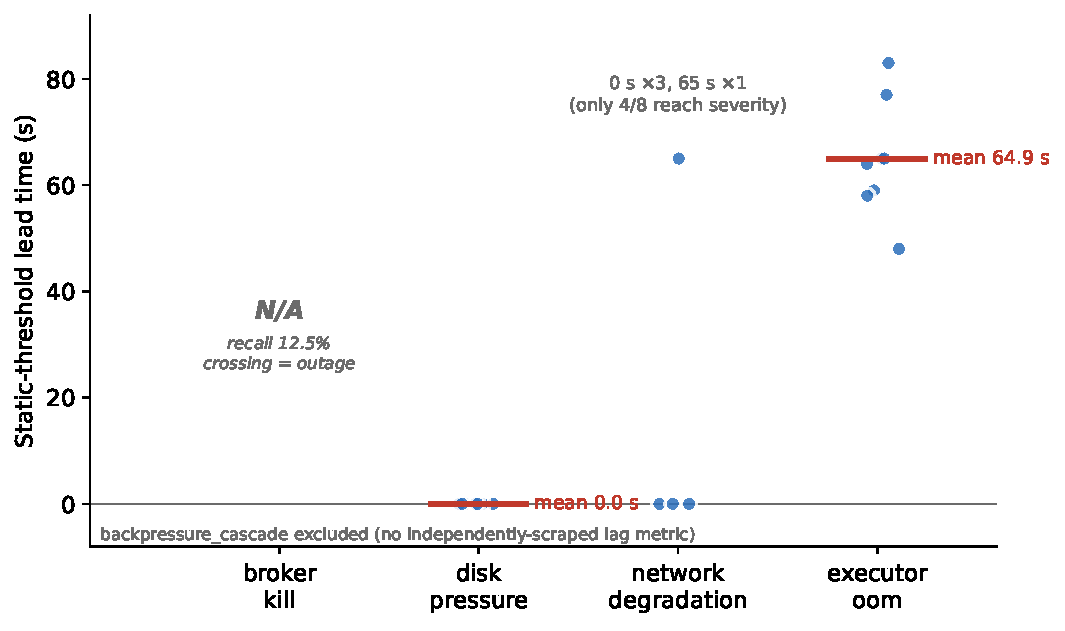
\includegraphics[width=\columnwidth]{figures/fig3-leadtime.pdf}
\caption{Static-threshold warning time by fault class: only \eo{}'s engineered ramp yields a real lead window (mean 64.9\,s); \dpr{} is 0\,s (8/8), \nd{} is 0\,s$\times$3 / 65\,s$\times$1 (4/8 reach severity), \bk{} is N/A.}
\label{fig:lead}
\end{figure}

\subsection{Sample-Size Robustness}
\eo{}'s negative result at $N=8$ raised whether eight episodes were simply too few. The collection was enlarged to 15 episodes under the identical protocol and re-evaluated. Of 15 raw episodes, 11 yielded a usable window. F1 rose to 0.909, but the trivial always-predict-pre-failure baseline rose with it to 0.957---the classifier still does not beat a constant prediction---and the permutation test placed the result at $p = 0.500$. Doubling the episode count moved neither the $p$-value (0.500 vs.\ 0.48 at $N=8$) nor the beats-trivial-baseline verdict; the null is not an artifact of insufficient statistical power. A genuinely settled pre-onset window was available for only two episodes, a structural consequence of the gradual-ramp protocol (each executor pod is 30--90 seconds old at the next episode's onset), not a sampling shortfall further collection would fix.

\section{Discussion}\label{sec:discussion}
\subsection{Answering the Research Questions}
The study asked four questions. Can models predict failure with a meaningful lead time? For this pipeline, no---no class produced a lead-time advantage. Which signals are most predictive, and does it vary by class? Only \dpr{} yielded a signal to attribute, and SHAP showed it rests on absolute magnitude rather than any precursor dynamic---so the honest answer is that no class exposed a genuinely predictive precursor signal in this telemetry. How does prediction quality vary across fault types? It is uniformly at chance except for \dpr{}'s mischaracterized case. Does ML outperform static-threshold alerting? Not on this pipeline: the one class where a static threshold gives real warning (\eo{}, 64.9\,s) is a class where the model is at chance, and the model's one significant result does not translate into operational lead time.

\subsection{Why a Null Result Here Is a Contribution}
That ML beats static thresholds is close to a foregone conclusion in the AIOps literature \cite{notaro2021,wu2021,lin2018}, and a paper that simply confirmed it would add little. The value of this result is the opposite: on a realistic, fully labeled Kafka--Spark pipeline, with ground-truth onset timestamps and honest significance testing, the expected advantage does not appear---and the one result that superficially shows it dissolves under mechanism verification. Two structural findings explain why. First, at a production-typical 60-second scrape interval, three of five fault classes progress from baseline to failure inside a single scrape step, leaving no intermediate telemetry for either a threshold or a model to act on; lead-time prediction is bounded by scrape cadence before it is bounded by model capacity. Second, only a deliberately engineered gradual ramp (\eo{}) creates a precursor window at all, and even there the static threshold already captures it---the model adds nothing. These are properties of the telemetry and the faults, and they will hold for any predictor, which is why reporting them matters.

\subsection{Positioning Against Closest Prior Work}
The result does not contradict Time Machine's lead-time prediction \cite{alharthi2023}: that system works on dense HPC event logs with far finer temporal resolution than 60-second Prometheus scrapes, and on naturally occurring failures rather than injected ones. It is consistent with, and extends, the recovery-focused streaming benchmark of Vogel et al.\ \cite{vogel2024}---where they show engine recovery behavior differs under injected faults, we show that the \emph{predictive} signal ahead of those faults is largely absent at standard scrape cadence. The mechanism-verification step is the methodological transfer we most want reused: none of the adjacent ML-failure-prediction studies \cite{wu2021,lin2018,harrison2018} reports per-instance ablation or SHAP cross-checking of \emph{why} a positive result holds, and had we not applied it, \dpr{}'s F1 = 0.941 would have been reported as a 98.6-second early-warning success.

\subsection{Limitations}
Three limitations bound the claims. The deployment is a single-node Kind cluster; behavior at production scale, with multiple brokers and executors and higher scrape resolution, is untested and could differ---particularly the scrape-cadence bound, which finer monitoring would relax. Sample sizes are small (8--15 episodes per class); the \eo{} enlargement showed the null is stable, but other classes were not similarly enlarged. The static-threshold baseline is calibrated on the same episodes it is evaluated on, so its recall reflects fit rather than generalization---appropriate for reproducing an operator's own-telemetry tuning, but not an out-of-sample claim. Each is a concrete target for replication rather than a reason to discount the benchmark.

\section{Conclusion}\label{sec:conclusion}
We built an open, reproducible fault-injection benchmark for failure prediction on a Kafka + Spark Structured Streaming pipeline, comprising infrastructure-as-code, five physically injected fault classes, a labeled dataset of 47 episodes with tooling-recorded onset timestamps, and a static-threshold baseline reproducing current alerting practice. Across three stock classifiers evaluated under leave-one-group-out cross-validation with permutation testing, only one of five fault classes produced a statistically significant classification signal, and mechanism verification showed even that signal to be an absolute-value discriminator rather than genuine precursor detection. No class yielded a machine-learning lead-time advantage over the threshold baseline, a null result stable across classifiers and across a doubling of one class's sample size. Two structural causes---the 60-second scrape cadence bounding available precursor telemetry, and only engineered gradual faults creating a precursor window a threshold already captures---explain the result and will constrain any predictor on similar telemetry. The benchmark, dataset, and the mechanism-verification methodology that caught this study's lone over-claim are released as reusable artifacts. Future work should relax the scrape-cadence bound with finer monitoring, replicate at multi-node production scale, and recover the excluded \bc{} class by adding independent Spark-lag instrumentation.

\section*{Acknowledgment}
% AI-DISCLOSURE (author decision required before submission — see the note delivered with this file):
% Portions of the text in this paper were drafted with the assistance of a large language model
% (Anthropic Claude), from the authors' own experimental data, results, and analysis; all content
% was verified and is the authors' responsibility. Retain, adjust, or remove per the target
% venue's current AI-use disclosure policy.
The authors used a large language model (Anthropic Claude) to assist in drafting portions of this manuscript from their own experimental data and analysis; the authors verified all content and are solely responsible for it.

\begin{thebibliography}{00}
\bibitem{kreps2011} J. Kreps, N. Narkhede, and J. Rao, ``Kafka: a distributed messaging system for log processing,'' in \textit{Proc. NetDB}, 2011.
\bibitem{armbrust2018} M. Armbrust, T. Das, J. Torres, B. Yavuz, S. Zhu, R. Xin, A. Ghodsi, I. Stoica, and M. Zaharia, ``Structured Streaming: a declarative API for real-time applications in Apache Spark,'' in \textit{Proc. ACM SIGMOD Int. Conf. Manag. Data}, 2018, pp. 601--613, doi: 10.1145/3183713.3190664.
\bibitem{salfner2010} F. Salfner, M. Lenk, and M. Malek, ``A survey of online failure prediction methods,'' \textit{ACM Comput. Surv.}, vol. 42, no. 3, pp. 1--42, 2010, doi: 10.1145/1670679.1670680.
\bibitem{notaro2021} P. Notaro, J. Cardoso, and M. Gerndt, ``A survey of AIOps methods for failure management,'' \textit{ACM Trans. Intell. Syst. Technol.}, vol. 12, no. 6, art. 81, 2021, doi: 10.1145/3483424.
\bibitem{zhang2024} L. Zhang, T. Jia, M. Jia, Y. Wu, A. Liu, Y. Yang, Z. Wu, X. Hu, P. S. Yu, and Y. Li, ``A survey of AIOps for failure management in the era of large language models,'' \textit{ACM Comput. Surv.}, 2024, doi: 10.1145/3746635.
\bibitem{wu2021} Z. Wu, H. Xu, G. Pang, F. Yu, Y. Wang, S. Jian, and Y. Wang, ``DRAM failure prediction in AIOps: empirical evaluation, challenges and opportunities,'' arXiv:2104.15052, 2021.
\bibitem{lin2018} Q. Lin, K. Hsieh, Y. Dang, H. Zhang, K. Sui, Y. Xu, J.-G. Lou, C. Li, Y. Wu, R. Yao, M. Chintalapati, and D. Zhang, ``Predicting node failure in cloud service systems,'' in \textit{Proc. ACM ESEC/FSE}, 2018, pp. 480--490, doi: 10.1145/3236024.3236060.
\bibitem{harrison2018} C. Harrison, C. R. Kirkpatrick, and I. Dutra, ``Bioinformatics computational cluster batch task profiling with machine learning for failure prediction,'' arXiv:1812.09537, 2018.
\bibitem{alharthi2023} K. A. Alharthi, A. Jhumka, S. Di, L. Gui, F. Cappello, and S. McIntosh-Smith, ``Time Machine: generative real-time model for failure (and lead time) prediction in HPC systems,'' in \textit{Proc. 53rd IEEE/IFIP Int. Conf. Dependable Syst. Netw. (DSN)}, 2023, pp. 508--521, doi: 10.1109/DSN58367.2023.00054.
\bibitem{basiri2016} A. Basiri, N. Behnam, R. de Rooij, L. Hochstein, L. Kosewski, J. Reynolds, and C. Rosenthal, ``Chaos engineering,'' \textit{IEEE Softw.}, vol. 33, no. 3, pp. 35--41, 2016, doi: 10.1109/MS.2016.60.
\bibitem{natella2016} R. Natella, D. Cotroneo, and H. Madeira, ``Assessing dependability with software fault injection: a survey,'' \textit{ACM Comput. Surv.}, vol. 48, no. 3, art. 44, 2016, doi: 10.1145/2841425.
\bibitem{chen2025} Z. Chen, M. Goudarzi, and A. Nadjaran Toosi, ``Resilience evaluation of Kubernetes in cloud-edge environments via failure injection,'' arXiv:2507.16109, 2025.
\bibitem{vogel2024} A. Vogel, S. Henning, E. Perez-Wohlfeil, O. Ertl, and R. Rabiser, ``A comprehensive benchmarking analysis of fault recovery in stream processing frameworks,'' in \textit{Proc. 18th ACM Int. Conf. Distrib. Event-Based Syst. (DEBS)}, 2024, doi: 10.1145/3629104.3666040.
\bibitem{alsayeh2020} H. Al-Sayeh, S. Hagedorn, and K.-U. Sattler, ``A gray-box modeling methodology for runtime prediction of Apache Spark jobs,'' \textit{Distrib. Parallel Databases}, vol. 38, pp. 819--839, 2020, doi: 10.1007/s10619-020-07286-y.
\bibitem{pham2025} L. Pham, H. Zhang, H. Ha, F. Salim, and X. Zhang, ``RCAEval: a benchmark for root cause analysis of microservice systems with telemetry data,'' in \textit{Companion Proc. ACM Web Conf. (WWW '25 Companion)}, 2025, pp. 777--780, doi: 10.1145/3701716.3715290.
\bibitem{breiman2001} L. Breiman, ``Random forests,'' \textit{Mach. Learn.}, vol. 45, no. 1, pp. 5--32, 2001, doi: 10.1023/A:1010933404324.
\bibitem{chen2016} T. Chen and C. Guestrin, ``XGBoost: a scalable tree boosting system,'' in \textit{Proc. 22nd ACM SIGKDD Int. Conf. Knowl. Discov. Data Min. (KDD)}, 2016, pp. 785--794, doi: 10.1145/2939672.2939785.
\bibitem{ke2017} G. Ke, Q. Meng, T. Finley, T. Wang, W. Chen, W. Ma, Q. Ye, and T.-Y. Liu, ``LightGBM: a highly efficient gradient boosting decision tree,'' in \textit{Adv. Neural Inf. Process. Syst. (NeurIPS)}, 2017, pp. 3146--3154.
\bibitem{lundberg2017} S. M. Lundberg and S.-I. Lee, ``A unified approach to interpreting model predictions,'' in \textit{Adv. Neural Inf. Process. Syst. (NeurIPS)}, 2017, pp. 4765--4774.
\end{thebibliography}

\end{document}
